\documentclass[a4paper, 16pt]{article}
\usepackage[UTF8]{ctex}
\usepackage{geometry}
\usepackage{graphicx}
\usepackage{setspace}
\usepackage{float}
\geometry{left = 1.0cm, right = 1.0cm, top = 2.0 cm, bottom = 2.5cm}
\title{编译原理第二章(一)}
\author{李鹏辉}

\begin{document}
\maketitle
\begin{flushleft}
1. (2.2.1)考虑下面的上下文无关文法:\\
\centerline{S $\rightarrow SS+ | SS* | a$}
1) 试说明如何使用该文法生成串 $aa+a*$\\
\centerline{$S \rightarrow SS* \rightarrow (SS+)S* \rightarrow aS+S* \rightarrow aa+S* \rightarrow aa+s*$}
\bigskip
2) 试为这个串构造一棵语法分析树\\
\begin{figure}[H]
\centering
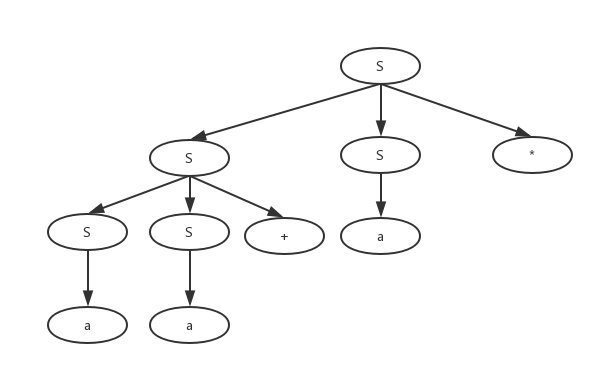
\includegraphics[scale = 0.6]{chapter2_hw1_1}
\caption{Parse tree 1.2}
\label{f1}
\end{figure}
3) 该文法生成的语言是什么?\\
该语言很难用形式化语言来描述,但简单而言表示以a为运算对象的加法和乘法的后缀表达式,并且加法和乘法的优先级相同。\\
\bigskip
4) 该文法具有二义性吗?为什么?\\
没有二义性,因为该语言是后缀(逆波兰)表达式,可以用堆栈实现,存在确定的算法算出数值来,并且所定义的加法和乘法,都是左结合。\\
\bigskip 
2. (2.2.5) 
1) 证明:用下面文法生成的所有二进制串的值都能被3整除。
\centerline{num $\rightarrow 11 | 1001 | num\,0 | num \, num$}

(1) 显然,对于 '11' 和‘1001’都能够被3整除\\
\begin{figure}[H]
\centering
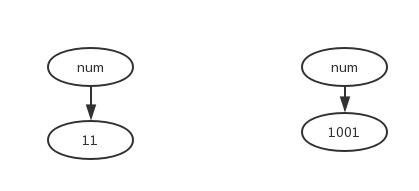
\includegraphics[scale=0.6]{chapter2_hw1_2}
\caption{Parse tree with two layers}
\label{f2}
\end{figure}
(2) 当该文法能够表示的数组Num >9时,根据文法的上述定义,可以知道,Num的语法树存在以下两种形式:
\begin{figure}[H]
\centering
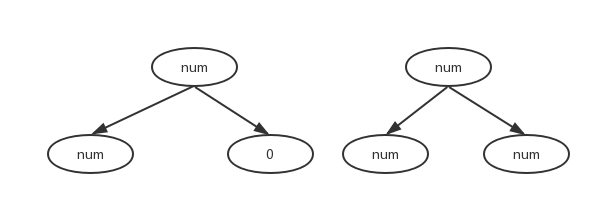
\includegraphics[scale=0.6]{chapter2_hw1_3}
\caption{Parse tree when Num $>$ 9}
\label{f2}
\end{figure}
用数学归纳法:\\
(1)语法分析树层数为2时,由上(1)知,能被3整除\\
(2)假设语法分析书层数为k时能够Num能够被3整除,只需要证明语法分析书层数为k+1时也能被3整除即可(k>=2)。\\
根据图 \ref{f2}可知,针对两种情况\\

 1. $Num = num * 2; num \%3 == 0; \Rightarrow $ Num \%3 == 0; \\
 2. $Num = num << bit\_len(num) + num; num\% 3 ==0; \Rightarrow Num \%3 ==0;$\\

综上所述, Num \%3 == 0;所以由该文法生成的语言能被3整除。\\
\bigskip
2) 上面的文法是否能够生成所有的能被3整除的二进制串?\\

能够举出反例证明存在数字串n能够被3整除,但不满足该文法。\\
$num = (10101)_2 = (21)_{10}$时,不属于该语言。
\bigbreak

3. (2.3.1)构造一个语法指导翻译方案,该方案把算术表示方式翻译为运算符在运算分量之前的前缀表示方式。例如-xy是表达式x-y的前缀表示。给出输入9-5+2和9-5*2的注释分析树。\\
中缀表达式到后缀表达式的语法制导,首先定义语义规则,保证没有二义性\\
\begin{table}[H]
\centering
\caption{definition}
\begin{tabular}{c|c}
\hline
$expr \rightarrow expr_1 + term$&$expr.t = '+' || expr_1.t || term.t$\\
$expr \rightarrow expr_1 - term$&$expr.t = '-' || expr_1.t || term.t$\\
$expr \rightarrow term$&$expr.t = term.t$\\

$term \rightarrow term_1 * factor$&$term.t = '*' || term_1.t || factor.t$\\
$term \rightarrow term_1 / factor$&$term.t = '/' || term_1.t || factor.t$\\
$term \rightarrow factor$&$term.t = factor.t$\\
$factor \rightarrow digit $&$factor.t = digit.t$\\
$factor \rightarrow (expr) $&$factor.t = (expr).t$\\
$digit \rightarrow$ 0 & $digit.t = '0'$\\
$digit \rightarrow$ 1 & $digit.t = '1'$\\
... & ...\\
$digit \rightarrow$ 9 & $digit.t = '9'$\\
\hline

\end{tabular}
\end{table}

\begin{figure}[H]
\centering
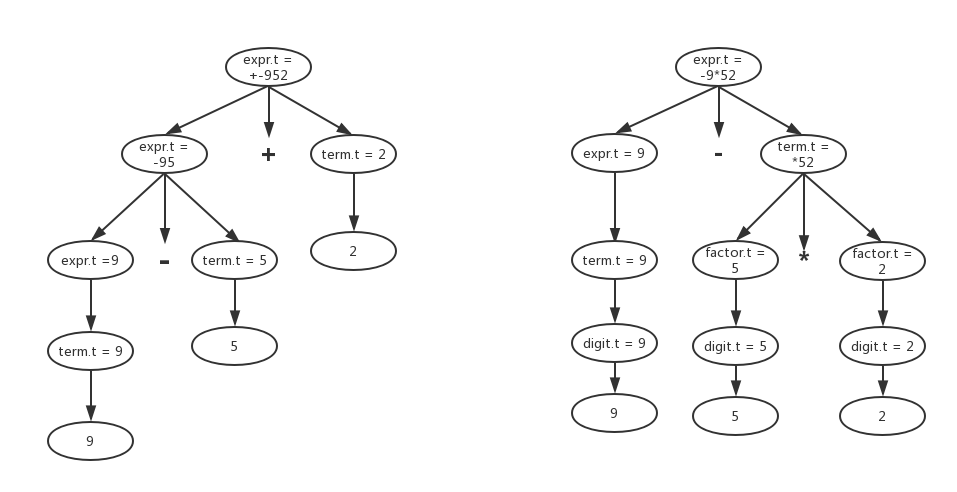
\includegraphics[scale=0.6]{chapter2_hw1_5}
\caption{Parse tree for 3}
\label{f3}
\end{figure}
\end{flushleft}
\end{document}

